\documentclass[12pt,a4paper,twoside,titlepage]{book}

\usepackage[italian]{babel}
\usepackage{hyperref}
\usepackage{tikz}
\usepackage{graphicx}
\usepackage{frontespizio}
\usepackage{listings}
\usepackage[Lenny]{fncychap}

\linespread{1.2}

\usetikzlibrary{automata, positioning, arrows}
\tikzset{->, >=stealth', node distance=5cm, initial text=$ $}

\begin{document}
\begin{frontespizio}
    \Universita{Verona}
    \Dipartimento{Scienze e ingegneria}
    \Corso{Ingegneria e Scienze informatiche}
    \Annoaccademico{2021--2022}
    \Titoletto{Tesi di laurea magistrale}
    \Titolo{Automazione di test di accettazione per dispositivi IoT embedded integrati nel cloud}
    \Candidato[VR432403]{Alessandro Righi}
    \Relatore{Mariano Ceccato}
\end{frontespizio}

\frontmatter

\tableofcontents

\mainmatter

\chapter{Introduzione}

Oggigiorno nelle nostre case ci sono sempre più prodotti connessi,
dalle lavatrici, ai televisori, fino agli impianti domotici che
consentono di controllare la nostra casa mediante un comando vocale
anche quando ci si trova dall'altra parte del pianeta.

Questi dispositivi svolgono anche funzioni critiche per il nostro
benessere domestico, quale ad esempio il controllo della temperatura
ambientale, che è oggetto del mio lavoro in IOTINGA.

IOTINGA s.r.l. nasce con lo scopo di aiutare altre aziende nel realizzare e
commercializzare disposivi IoT. IOTINGA si distingue dagli altri
concorrenti per un'attenzione particolare alla componente software,
in tutte le sue sfaccettature, dall'interazione fisica con le perferiche
hardware, alla gestione del dato mediante un'infrastruttura realizzata
con tecnologie cloud serverless, fino alla sua presentazione ai consumatori,
mediante realizzazione di applicazioni Android/iOS.

La mia esperienza in IOTINGA inizia nel Febbraio 2020. In questi 3 anni
ho avuto l'occasione di vedere cresce l'azienda, e fornire il mio conributo
nello sviluppo del progetto ``IRSAP NOW'', che ho avuto modo di seguire
in prima persona fin dalla sua fase embrionale.

IRSAP NOW è l'ecosistema domotico che integra al proprio interno tutti
i prodotti connessi di IRSAP s.p.a., una grande impresa rodigina leader
nel settore del comfort termico. Storicamente produttrice di radiatori,
inventrice del termoarredo, si distingue oggi per prodotti dal design altamente
ricercato, non che dall'elevato contenuto tecnologico, quali impianti VMC,
radiatori elettrici connessi, e sistemi di gestione remota di impianti di riscaldamento.

\section{Il progetto IRSAP radiatore elettrico}

All'interno di questa piattaforma si innesta il prodotto in esame,
ovvero la gamma di radiatori elettrici connessi IRSAP. Il catalogo si compone di
decine di prodotti, uno su tutti il ``Polygon''(\autoref{fig:polygon}), vincitore del
``CES Best of Innovation 2022'' (\autoref{fig:ces}) nella categoria Home Appliances,
nonché di altri prestigiosi premi a livello internazionale, quali ``Red Dot Design'',
``German Design'', ``AIFA'' % TODO,
grazie al suo design innovativo ed al suo contenuto tecnologico,
a cui noi di IOTINGA abbiamo contribuito.

\begin{figure}[ht]
    \centering
    
\includegraphics[width=12cm]{img/polygon.jpeg}
    \caption{Polygon}
    \label{fig:fig:polygon}
\end{figure}

``Polygon'' è dotato internamente di elettronica in grado di connettersi mediante
Wi-Fi direttamente al cloud ``IRSAP NOW'', ed integra oltre alla funzione scaldante
anche un'illuminazione ambientale LED colorati.

Mi sono occupato in prima persona dello sviluppo del firmware del dispositivo nella
sua interezza, mentre alcuni colleghi hanno seguito la parte di progettazione hardware
e di integrazione all'interno dell'ecosistema cloud e della app.

\begin{figure}[ht]
    \centering
    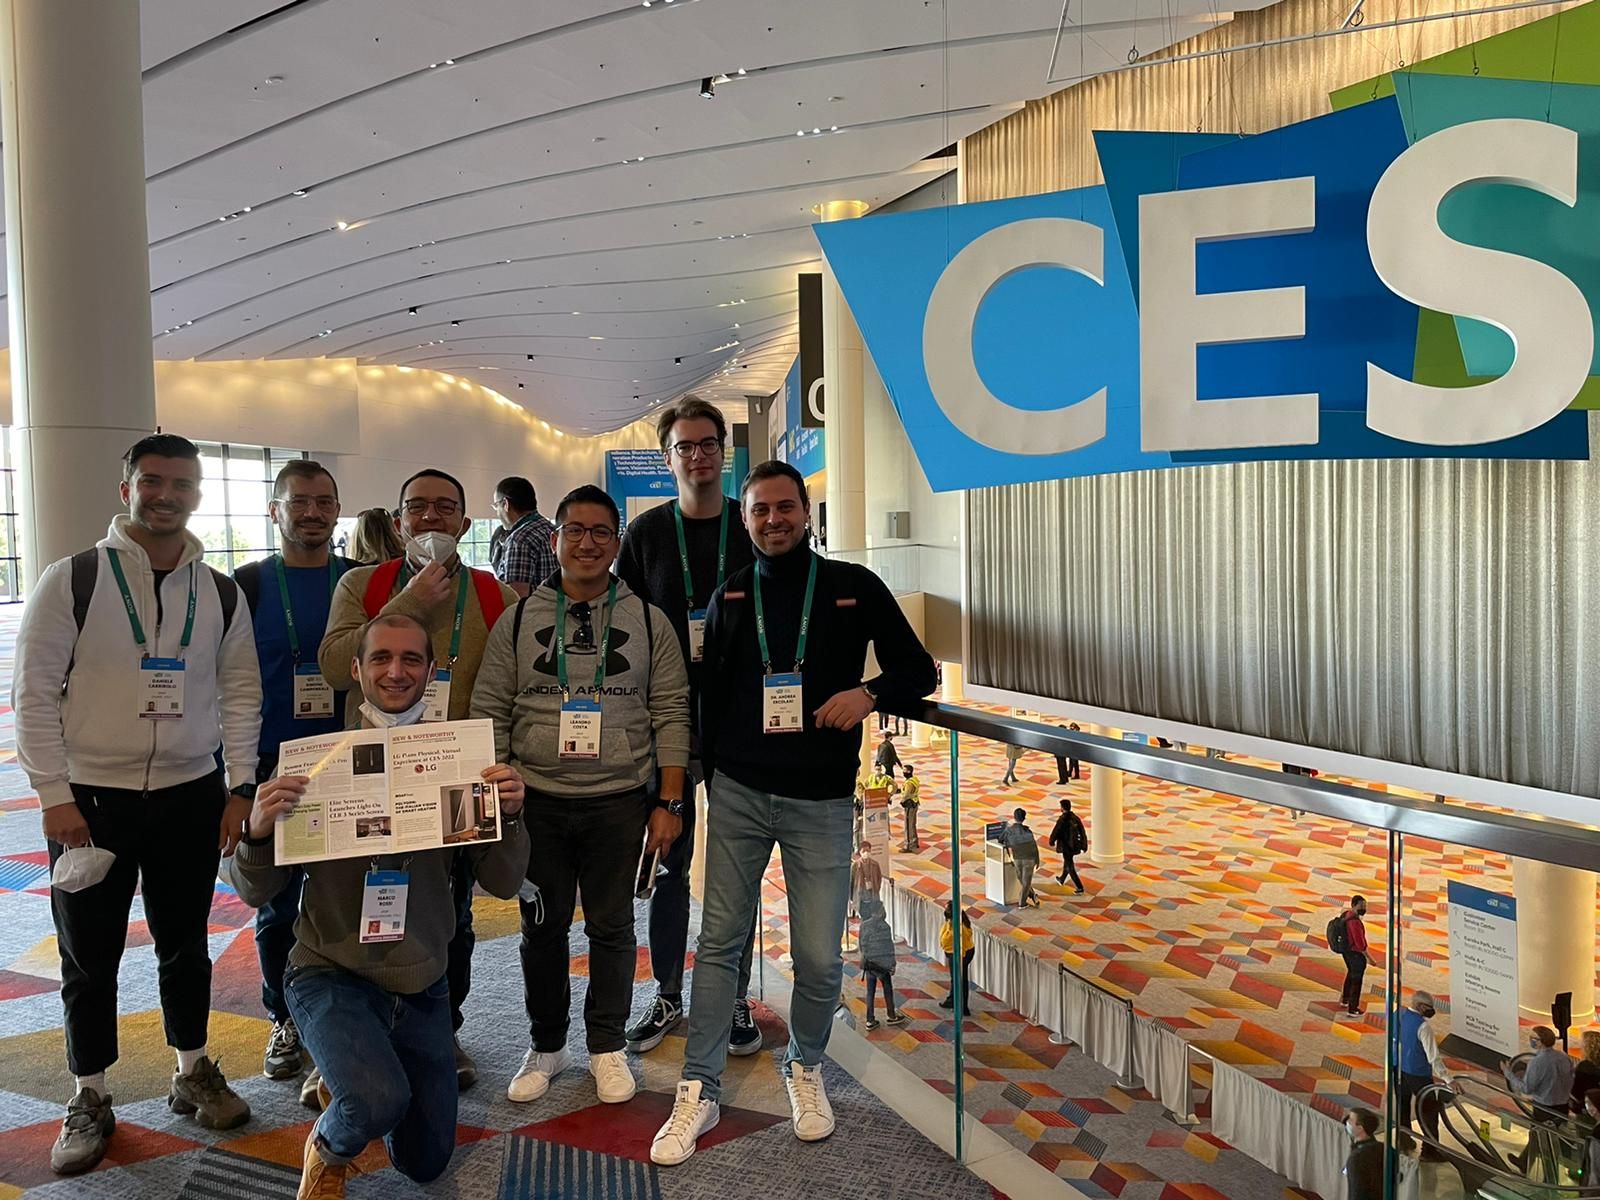
\includegraphics[width=12cm]{img/ces.jpeg}
    \caption{IRSAP ed IOTINGA al CES 2022}
    \label{fig:fig:ces}
\end{figure}

\section{Motivazioni (diffcolta' testing IoT/cloud)}

La caratteristica fondamentale per questi prodotti è l'affidabilità.
Infatti nessun utente installerebbe in casa propria un dispositivo che
non è in grado di svolgere la funzione per la quale è stato acquistato.

A maggior ragione i danni derivanti dal malfunzionamento di un impianto
di riscaldamento possono coinvolgere non solo cose ma anche estendersi
a persone ed animali domestici.

È tassativo prestare attenzione alle problematiche che si possono verificare
in utenza, le quali non sono solo un danno per il cliente stesso ma anche
per l'azienda produttrice:

\begin{itemize}
\item la prima impressione sul cliente è quella che conta, se il cliente si ritrova
    un prodotto che funziona male o addira non svolge la funzione prevista ne parlerà
    male, anche mediante recensioni negative online, e creerà un danno d'immagine all'azienda
    difficilissimo da sanare
\item quando il problema si verifica dal cliente è complicata la diagnostica. I clienti,
    e spesso anche gli installatori stessi, non hanno competenze tecniche o il
    tempo da dedicare nel supportare il produttore nella ricerca del problema
\item se il problema non è risolvibile mediante un aggiornamento firmware è necessario
    effettuare un reso, che ha dei costi molto elevati per il produttore, in quanto
    durante il trasporto molto spesso il prodotto viene danneggiato e quindi deve
    essere rimpiazzato con un nuovo
\end{itemize}

È di fondamentale importanza assicurarsi di identificare il prima possibile quanti
più problemi possibili prima che il prodotto arrivi nelle mani dell'utente finale.

In tutto questo il software ricopre un ruolo sempre più da protagonista, in quanto
per garantire la connettività al cloud è necessario gestire una complessità elevata.

I prodotti della precedente generazione utilizzavano il software per una mera gestione
delle periferiche fisiche del prodotto, senza la necessità di interfacciarsi con sistemi
terzi. Al contrario i prodotti della attuale per svolgere tutte le funzioni di
integrazione cloud in maniera sicura richiedono un livello aggiuntivo di astrazione,
ovvero quello di un RTOS (sistema operativo real-time).

Anche l'hardware stesso è più evoluto, infatti si passa dalle piattorme ad 8 bit ai
microcontrollori a 32, con funzionalità sempre più assimilabili a quelle di un sistema
general purpose, quali ad esempio una gestione di programmazione concorrente, uno
stack di rete TCP/IP, ed una gestione della memoria virtual con MMU.

Un'altra differenza rispetto al passato è la possibilità di aggiornare il software dopo
che il prodotto lascia la fabbrica, mediante aggiornamenti di tipo ``Over The Air'' (OTA).
Questo si rende necessario non solo per la mera introuduzione di nuove funzionalità in
un prodotto esistente, ma anche per mantenere il software al passo con l'evoluzione degli
altri sistemi a cui esso si collega, quale ad esempio modifiche nei protocolli di rete
dettate dall'arrivo di nuovi standard.

Sebbene l'aggiornamento consenta di risolvere problemi dopo che il dispositivo ha lasciato la
fabbrica esso comporta anche una criticità, in quanto vi è il rischio di introdurre altri problemi
in prodotti che fino a quel momento non li avevano, andando a creare un disservizio.

Bisogna infine tener conto che un prodotto di questo tipo segue un ciclo di vita molto lungo
rispetto ad esempio a PC o smartphone, che può tranquillmente superare i 10 anni dalla data di
immissione nel mercato, e l'utente si aspetta che in tutti questi anni possa continuare ad
utilizzarlo come il giorno in cui lo ha acquistato.

Conseguentemente diventa prioritario garantire i massimi livelli di qualità possibile
sul software rilasciato. Questo non si limita alla semplice assenza di bug, in quanto
questa è una garanzia che matematicamente è impossibile offrire, ma anche all'adottare
delle procedure procedure tali che consentano, dal momento che un bug si
presenta, di individuarlo e sistemarlo nel minor tempo possibile.

Tracciabilità e mantenibilità del codice sono quindi parole chiave, la prima garantisce che
sia sempre possibile risalire all'esatta versione del codice per il quale viene segnalato un
problema di modo da poterlo riprodurre, la seconda invece assicura che la soluzione al problema
sia implementabile nel minor tempo possibile e senza il rischio di regressioni.

Infine l'altro punto cardine è l'eseguire test metodologici prima che il firmware venga
rilasciato al pubblico, sia tramite aggiornamento OTA che tramite installazione in fabbrica
su di un nuovo prodotto.

\subsection{Prassi attuale testing}

Allo stato attuale abbiamo 3 momenti di validazione:

\begin{enumerate}
    \item test da parte dello sviluppatore
    \item test di accettazione interna (in IOTINGA)
    \item test di accettazione del cliente finale (IRSAP)
\end{enumerate}

\subsection{Test di sviluppatore}

Quando uno sviluppatore finisce di implementare una nuova funzionalità o risolve un
bug  prima di considerare l'attività conclusa ed integrare il
proprio lavoro nel ramo di sviluppo principale ed effettua i propri test.

Questi si occupano sia di verificare che quanto è stato implementato è conforme
alla specifica approvata dal cliente (nel caso di nuove funzionalità) oppure che
il bug sia stato risolto, sia che non siano stato modificato il funzionamento del sistema
nelle parti che sono state impattate dalla modifica.

Tali test sono a discrezione dello sviluppatore, che avendo modificato il codice sa
quali comportamenti sono impattati dalla modifica che ha realizzato e quindi devono essere
provati.

Questi test possono essere automatizzati facilmente mediante la creazione di unit-test.

\subsection{Test di accettazione interna}

Questi test sono effettuati prima di ogni rilascio di un nuovo artefatto verso il cliente.

Si occupano di validare che il software garantisca il funzionamento di una serie di casi d'uso critici,
senza i quali il sistema non sarebbe utilizzabile.
Solo se una versione del software passa tutti questi test può essere consegnata al cliente.

Essi si pongono dal punto di vista dell'utente finale, pertanto sono effettuati su un
hardware completo, isolato però dal resto del sistema, ovvero dalla componente cloud
e dall'applicazione mobile. Questo per evitare che vi sia il dubbio che il bug sia
nel cloud o nella app anziché nel dispositivo stesso.

Attualmente vengono effettuati seguendo un documento contenente una serie di passi, ognuno
idicante:

\begin{itemize}
    \item azione: un'operazione da effettuare sul sistema mediante l'interazione fisica
        con il dispositivo (pressione di pulsanti) oppure mediante cloud (tramite un'apposito
        strumento che consente di simulare i messaggi inviati dal cloud e dalla app)
    \item risultato atteso: postcondizioni da verificare dopo aver effettuato l'azione, ad
        esempio ``i led sono rossi'' oppure ``entro 5 secondi viene inviato al cloud un messaggio''.
        Nel caso la postcondizione sia verificata è possibile procedere al passo successivo, altrimenti
        il test viene interrotto con esito negativo, e deve essere segnalato ad uno sviluppatore il problema.
\end{itemize}

Preferibilmetne questa procedura viene fatta eseguire da chi non ha preso parte allo
sviluppo del sistema stesso. Questo per evitare che chi esegue la procedura, conoscendo
le logiche interne del software, possa essere portato a saltare o ignorare determinati
passaggi in quanto ``ovvi'', mentre chi non conosce il sistema è più propenso a seguire
i passaggi alla lettera e segnalare ogni singolo comportamento discordante con quanto
atteso.

\subsection{Test di accettazione del cliente finale}

Sul cliente finale ricade la responsabilità (anche a livello legale) del prodotto
che viene immesso sul mercato con il proprio nome sopra, e questo include anche
il software. Questo comporta il fatto che a sua volta deve svolgere dei test per
assicurarsi che il software sia conforme a quanto atteso, e nel caso segnalare i
problemi riscontrati in maniera tale che vengano corretti.

Questi test sono volti a testare tutte le funzionalità del prodotto in tutte le loro
possibili configurazioni, anche mediante l'ausilio di strumentazione altamente
specializzata quali camere climatiche per valutarne l'efficacia di termoregolazione.

Nel caso questi test abbiano successo l'artefatto testato passa da stato di candidato
al rilacio a produzione, e viene quindi installato in fabbrica su tutti i nuovi radiatori
prodotti, nonché viene lanciato un aggiornamento OTA su tutti i dispositivi già installati
presso i clienti finali.

\section{Possibilità di automatizzare il testing}

Dopo questa panoramica sulle tre attuali fasi di test ci concentreremo sui test
descritto al secondo punto, ovvero i test di acettazione fatti internamente a IOTINGA.

La scelta è ricaduta su di essi in quanto:
\begin{itemize}
    \item i test svolti dal singolo sviluppatore sono a propria discrezione, e quantomeno
        per la regressione sono facilmente automatizzabili in modi classici quali gli unit test
    \item i test svolti da IRSAP sono fuori dal nostro controllo, in quanto il cliente
        li svolge a propria discrezione
\end{itemize}

L'approccio attuale, basato sul documento di test con fasi da seguire, presenta
alcune problematiche:
\begin{itemize}
    \item la procedura è ripetitiva, e questo può facilmente introdurre
        l'operatore che esegue i test a commettere errori, con dolo o meno
    \item il fatto che la procedura è eseguita manulmente è un costo in termini di
        tempo per l'azienda
    \item il fatto che sia un costo porta la procedura ad essere per forza di cose
        limitata sia nel numero di scenari che sono effettivamente testati sia nel
        numero di build testate (il che limita il numero di rilasci che vengono
        fatti verso il cliente finale, preferendo di accorpare più modifiche in un
        singolo rilascio per effettuare un solo ciclo di test)
\end{itemize}

Vediamo quindi che automatizzare questa parte con un meccanismo di testing automatico
può essere un risultato interessante per gli scopi dell'azienda, in grado di far
risparmiare del tempo, sia perché i test non sono più svolti manualmente, sia perché
testando più scenari si riduce la probabilità che un bug sfugga e finisca nelle mani
del cliente finale. Inoltre questo ultimo punto evita anche danni all'immagine dell'azienda
causati dal rilascio di un software che presenta non conformità.

\chapter{Related work}
\section{Tool commerciali/open-source}

%% TODO: here

\chapter{Approccio}

Prima di descrivere come si è scelto di implementare l'automatizzazione della fase
di validazione del software è necessario fare un breve excursus per descrivere nei
dettagli il sistema che vogliamo testare.

\section{Caratteristiche hardware}

Il radiatore elettrico contiene al suo interno una scheda elettronica, che viene
attualmente prodotta in due modelli differenti:
\begin{itemize}
    \item \textit{luxury}: è la versione più basilare che consente di gestire le
        funzionalità base del radiatore, ossia la regolazione della temperatura ambiente
    \item \textit{design}: è la versione riservata ai prodotti di alta gamma. Offre, in
        aggiunta a tutto quanto offerto dalla \textit{luxury}, un sensore di qualità
        dell'aria (in grado di rilevare i valori di VOC e CO2) e la possibilità di
        controllare una striscia LED RGBW, utilizzata in alcuni radiatori per questioni
        di illuminazione estatica.
\end{itemize}

Inoltre a parità di elettronica un radiatore può o meno avere a disposizione le
seguenti funzionalità:
\begin{itemize}
    \item Fil Pilote: uno standard francese per l'interconnessione dei radiatori ad una
        centralina di controllo mediante un secondo ingresso di segnale a 230V
    \item LED RGBW: disponibili solo su radiatore con scheda design, consente di
        illuminare l'ambiente circostante al radiatore per creare atmosfera
\end{itemize}

Tutte le versioni di scheda elettronica eseguono la stessa versione del firmware,
che ha una fase iniziale in cui identifica la tipologia di scheda e le funzionalità
opzionali abilitate leggendole da un file di configurazione caricato nel dispositivo
in fase di collaudo, e di conseguenza configura le periferiche del microcontrollore.

Tuttavia per essere esaustivi è necessario svolgere i test di accettazione su entrambe
le versioni di scheda elettronica, in quanto possono esservi comportamenti differenti.

Il cuore del sistema è un microcontrollore Wi-Fi della Telit, il GS2200M, che presenta
le seguenti caratteristiche:

\begin{itemize}
    \item processore dual core ARM Cortex M3 fino a 120Mhz, di cui un core dedicato
        alla gestione del Wi-Fi ed uno all'esecuzione dell'applicativo
    \item 1Mb di RAM in totale, di cui all'incirca 500kB utilizzabile dall’applicazione,
        il resto dedicata all'uso della parte Wi-Fi
    \item 4Mb di memoria flash interna, in parte dedicata al codice del firmware ed
        in parte come filesystem interno in cui memorizzare i dati dell'applicazione
    \item interfaccia Wi-Fi b/g/n a 2.4Ghz in grado di operare sia in modalità station
        (client) sia che access-point (AP) a cui connettersi direttamente
    \item 19 input/output digitali
    \item 3 output PWM
    \item 2 ingressi analogici mediante ADC, uno a 10 ed uno a 12 bit
    \item un interfaccia I2C hardware
    \item un interfaccia SPI hardware
    \item due interfacce seriali UART
    \item modulo RTC interno
\end{itemize}

Tale microcontrollore si interfaccia con le seguenti periferiche hardware presenti
sulla scheda madre:

\begin{itemize}
    \item una resistenza (cartuccia) a 230V che provvede a riscaldare il fluido
        termoconduttivo presente all'interno del radiatore
    \item una sonda di temperatura NTC usata per rilevare la temperatura ambiente
    \item una pulsantiera dotata di due pulsanti capacitivi e dei led RGB di illuminazione
        come feedback verso l'utente
    \item un buzzer utilizzato per dare un feedback uditivo all'utente
    \item solo per le schede ``design'' un sensore di qualità dell'aria in grado di
        misurare i livelli VOC e CO2
    \item solo per i modelli che lo prevedono un ingresso per il segnale ``Fil Pilote''
    \item solo per i modelli che li prevedono una striscia a led RGBW di illuminazione ambientale
    \item sempre solo per alcuni modelli una seconda sonda di temperatura in grado di
        misurare la temperatura del corpo riscaldante, in maniera tale da migliorare
        l'accuratezza degli algoritmi di termoregolazione
\end{itemize}

\section{Caratteristiche software}

Il firmware eseguito sul dispositivo è scritto in linguaggio C.

Il produttore fornisce un SDK basato sull'ambiente di sviluppo e compilatore IAR,
che offre le seguenti componenti:

\begin{itemize}
    \item un sistema operativo real-time (\textit{RTOS}) basato su ThreadX
    \item uno stack TCP/IP basato su NetX
    \item libreria di gestione della connessione Wi-Fi
    \item filesystem
    \item libreria TLS
    \item client e server HTTP/s
    \item aggiornamento OTA con doppia partizione
\end{itemize}

Il firmware è essenzialmente suddiviso in 4 moduli (task):

\begin{itemize}
    \item \textit{termostato}, task che si occupa di tutto quel che è necessario
        per regolare la temperatura ambiente secondo le modalità di funzionamento del dispositivo,
        della lettura delle sonde ambiente/VOC, non che della gestione dell'illuminazione LED
        nel caso sia presente
    \item \textit{AWS}, si occupa di mantenere la connessione MQTT verso AWS IoT Core,
        sincronizzato lo stato interno del dispositivo con il server ``IRSAP NOW'' mediante protocollo MQTT
    \item \textit{hmi}, si occupa di rispondere agli input dell'utente
        sulla pulsantiera e di darne relativo feedback mediante l'uso dei LED RGB e del buzzer
    \item \textit{HTTP}, si occupa di fornire mediante webserver HTTP un'API REST con
        la quale è possibile interagire direttamente con il dispositivo. È utilizzata
        per la fase di provisioning.
\end{itemize}

\subsection{Stati interni del dispositivo}

Il dispositivo ad alto livello può trovarsi in 3 stati distinti:

\begin{itemize}
    \item \textit{non abbinato}: in attesa di un primo abbinamento da app. Ogni funzione del
        dispositivo è esclusa finché l'utente non lo collega mediante l'applicazione
    \item \textit{disconnesso}: il dispositivo è stato in passato abbinato ma al momento non è
        connesso al cloud, perché ad esempio la connessione Wi-Fi non è momentaneamente disponibile
    \item \textit{connesso}: il dispositivo è connesso e sincronizzato con il cloud
\end{itemize}

\begin{figure}[ht]
    \centering
    \begin{tikzpicture}
        \node[state] (unbounded) {Non abbinato};
        \node[state, below left of=unbounded, below=1cm] (offline) {Disconnesso};
        \node[state, right of=offline] (online) {Connesso};
        \draw (unbounded) edge[bend left, align=left, right] node{abbinato\\con successo} (online)
        (offline) edge[bend left, above] node{connessione} (online)
        (offline) edge[bend left, left, align=right] node{ripristino\\di fabbrica} (unbounded)
        (online) edge[bend left, below] node{disconnessione} (offline)
        (online) edge[bend left, align=right, right] node{ripristino\\di fabbrica} (unbounded);
    \end{tikzpicture}
    \caption{Stati del radiatore}
    \label{fig:stati}
\end{figure}

Ad ogni stato del dispositivo corrisponde l'attivazione/disattivazione di uno o più
componenti software del dispositivo:

\begin{center}
\begin{tabular}{| c | c | l |}
    \hline
    stato & modo Wi-Fi & moduli attivi \\
    \hline
    \textit{non abbinato} & AP & HMI, HTTP \\
    \hline
    \textit{disconnesso} & client & HMI, termostato \\
    \hline
    \textit{connesso} & client & HMI, termostato, AWS \\
    \hline
\end{tabular}
\end{center}

\subsection{Termoregolazione}

La componente di termoregolazione si occupa di regolare la temperatura ambiente portandola
il più vicino possibile a quanto desiderato dall'utente (set-point) mediante
il controllo dell'accensione (on/off) dell'elemento riscaldante. Il feedback sulla
temperatura ambiente è ottenuto mediante la sonda di temperatura NTC.

Il dispositivo ha diversi modi di funzionamento:
\begin{itemize}
    \item standby: dispositivo completamente spento, sia per quanto riguarda il riscaldamento
        che per l'illuminazione LED
    \item antigelo: il dispositivo mantiene una temperatura di sicurezza (impostata dall'utente)
        per prevenire danni dati da una tempratura ambiente troppo bassa (ad es. congelamento delle tubature)
    \item vacanza: all'interno di un intervallo temporale impotato dall'utente funziona
        in modalità antigelo
    \item away: imposta un set-point ridotto (ECO) in quanto l'utente non è in casa
    \item programmato: segue una programmazione settimanale che consente per ogni
        giorno della settimana di creare fino ad 8 fasce orarie
    \item manuale temporaneo: segue un set-point manuale per un determinato tempo
    \item manuale: segue il set-point utente che è fisso e non varia mai
        configurato dall'utente, quindi torna a funzionare nella modalità precedente
    \item fil pilote: il dispositivo è controllato (ove disponibile) da un segnale
        esterno in ingresso sul cavo fil pilote
\end{itemize}

È possibile mediante interfaccia utente muoversi fra le varie modalità come dettagliato
in \autoref{fig:modi}.

\begin{figure}[ht]
    \centering
    \begin{tikzpicture}
        \node[state] (programmato) {Programmato};
        \node[state, right of=programmato, align=center] (manuale-tempo) {Manuale\\temporaneo};
        \node[state, right of=manuale-tempo] (manuale) {Manuale};
        \draw (manuale) edge[loop above] node{modifica set-point} (manuale)
            (programmato) edge[bend left, above] node{modifica set-point} (manuale-tempo)
            (manuale-tempo) edge[bend left, above] node{modifica set-point} (manuale);
    \end{tikzpicture}
    \caption{Modi del radiatore}
    \label{fig:modi}
\end{figure}

\subsection{Comunicazione cloud}

La componente cloud è implementata su AWS. La connessione avviene grazie al protocollo
MQTT usando il servizio broker di AWS, IoT Core.

La connessione è cifrata mediante TLS ed autenticata mediante certificato TLS client
specifico per il singolo dispositivo, generato e programmato nel dispositivo in fase
di produzione della scheda elettronica da una CA intermedia a sua volta firmata dalla
CA root di AWS come in \autoref{fig:tls-chain}.

\begin{figure}[ht]
    \centering
    \begin{tikzpicture}
        \node[rectangle, draw, minimum height=1cm] (root) {root CA AWS};
        \node[rectangle, draw, right of=root, align=center, minimum height=1cm] (intermedia) {CA intermedia\\ produttore};
        \node[rectangle, draw, right of=intermedia, minimum height=1cm] (dispositivo) {certificato dispositivo};
        \draw (root) edge[above] node{firma} (intermedia)
            (intermedia) edge[above] node{firma} (dispositivo);
    \end{tikzpicture}
    \caption{Catena TLS}
    \label{fig:tls-chain}
\end{figure}

Per quanto concerne il protocollo di comunicazione in origine abbiamo valutato il
protocollo Device Shadowing\footnote{\url{https://docs.aws.amazon.com/it\_it/iot/latest/developerguide/iot-device-shadows.html}} supportato nativamente da AWS IoT Core. Tuttavia, tale
protocollo aveva delle limitazioni che non ne consentivano l'utilizzo nella nostra
applicazione, in particolare:

\begin{itemize}
    \item il pacchetto viene codificato in JSON, il che presenta un overhead di memoria
        e CPU notevole per il microcontrollore scelto. Inoltre la codifica JSON può
        introdurre dei bug di encoding
    \item vi è un hard-limit di 8Kb di dimensione massima di un documento di stato (shadow).
        Questo, seppur poteva essere sufficiente nelle prime versioni del prodotto, andava
        a limitare possibilità di espansione futura del prodotto
    \item il protocollo di comunicazione trasferisce dei delta, che sebbene riducano la
        dimensione di un pacchetto di dati rendono più complessa la sincronizzazione degli
        stati del sistema
\end{itemize}

Per tutte queste ragioni abbiamo scelto di adottare un protocollo binario proprietario,
tramite il quale andiamo a trasferire stati completi del dispositivo.

Abbiamo deciso di mantenere comunque i concetti di alto livello dati dal protocollo AWS
Device Shadowing, per tanto identifichiamo come:
\begin{itemize}
    \item \textit{state desired} come lo stato in cui si vuole portare il dispositivo, ovvero le
        impostazioni che l'utente può modificare agendo dalla app, quali ad esempio la modalità di funzionamento,
        la programmazione oraria, la configurazione dei LED RGB, etc.
    \item \textit{state reported} lo stato attuale del dispositivo. È un superset dello stato
        desired, in quanto oltre a tutti i campi di quest'ultimo include anche tutti quei valori
        in sola lettura (ovvero che solo il dispositivo può modificare), ovvero i parametri
        statistici e di monitoraggio quali la temperatura ambiente, il livello di qualità dell'aria (VOC),
        gli allarmi del dispositivo, la qualità della connessione Wi-Fi, etc.
\end{itemize}

Il protocollo è quindi stateless, e consente di effettuare 4 messaggi, più relative risposte,
(come visibile in \autoref{fig:comunicazione_cloud}):

\begin{itemize}
    \item \textit{get}: disponibile fra dispositivo e cloud, consente la richiesta dello stato \textit{desired} corrente
    \item \textit{reported-update}: disponibile fra dispositivo e cloud, trasmette lo stato
        completo del dispositivo al server
    \item \textit{delete}: eliminazione dello stato corrente presente su cloud
    \item \textit{desired-udpate}: unico messaggio inviato dal cloud al dispositivo,
        trasmette lo stato completo desired
\end{itemize}

Il tipo di messaggio dipende dal topic MQTT sul quale i pacchetti sono pubblicati. Ad
un messaggio pubblicato dal dispositivo verso il server il server risponde in base allo
stato della richiesta sullo stesso topic con aggiunto un suffisso:
\begin{itemize}
    \item /accepted: la richiesta è stata accettate
    \item /rejected: la richiesta è stata respinta dal server
\end{itemize}

\begin{figure}[ht]
    \centering
    \begin{tikzpicture}
        \node[rectangle, minimum height=1cm, draw] (dispositivo) {Radiatore Elettrico};
        \node[rectangle, minimum height=1cm, draw, right of=dispositivo] (cloud) {Cloud AWS};
        \draw (dispositivo) edge[bend left=40, above] node{\textit{get}} (cloud)
            (dispositivo) edge[bend left=10, above] node{\textit{reported-update}} (cloud)
            (dispositivo) edge[bend right=10, below] node{\textit{delete}} (cloud)
            (cloud) edge[bend left=40, below] node{\textit{desired-update}} (dispositivo);
    \end{tikzpicture}
    \caption{Schema di comunicazione dispositivo/cloud}
    \label{fig:comunicazione_cloud}
\end{figure}

Il client può identificare a quale richiesta fa riferimento ad una risposta attraverso un
token (clientToken) che il client setta su ogni richiesta inviata e che il server aggiunge
ad ogni risposta che invia al client.

Di base ogni messaggio prevede un header fisso che include i seguenti campi:

\begin{center}
\begin{tabular}{| l | c | l |}
    \hline
    \textbf{campo} & \textbf{byte} & \textbf{descrizione} \\
    \hline
    timestamp & 4 & timestamp di invio del messaggio \\
    \hline
    clientToken & 4 & stringa random scelta dal client \\
    \hline
    version & 4 & versione del messaggio \\
    \hline
    length & 2 & lunghezza totale del messaggio (header incluso) \\
    \hline
    type & 1 & tipo di messaggio, identifica il payload presente \\
    \hline
\end{tabular}
\end{center}

A seguire nel messaggio è presente il payload.

\subsection{API di configurazione locale}

Quando il dispositivo viene acceso per la prima volta è necessario fornirgli la
configurazione della rete Wi-Fi e l'identificativo (UUID) dell'impianto al quale
collegarsi prima che esso possa iniziare a funzionare.

Per fare ciò il dispositivo mette a dispozione un'API REST attraverso la quale la
app ``IRSAP NOW'' comunica attraverso una connessione Wi-Fi diretta (in questa fase
il dispositivo imposta la propria interfaccia Wi-Fi in modo access-point).

Mette a dispozizione le seguenti API REST:

\begin{center}
\begin{tabular}{| l | c | l |}
    \hline \textbf{endpoint} & \textbf{metodo} & \textbf{descrizione} \\
    \hline /irsap/state & GET & ottiene lo stato corrente del dispositivo \\
    \hline /irsap/wifi/scan & GET & ottiene l'elenco di reti Wi-Fi visibili dal dispositivo \\
    \hline /irsap/provision & POST & invia al dispositivo la configurazione \\
    \hline /irsap/test & POST & attiva la modalità collaudo del dispositivo \\
    \hline /gainspan/system/fwup & POST & invia un aggiornamento firmware al dispositivo \\
    \hline
\end{tabular}
\end{center}

\subsection{HMI}

L'interfaccia untente del dispositivo si compone di due pulsanti, \textbf{+} e \textbf{-},
i LED RGB di illuminazione della pulsantiera ed il buzzer.

Tramite l'HMI è possibile affettuare le seguenti operazioni:

\begin{itemize}
    \item pressione breve \textbf{+}: incrementa il set-point corrente
    \item pressione breve \textbf{-}: decrementa set-point corrente
    \item pressione per più di 3 secondi (ma meno di 5) del tasto \textbf{-}:
        attiva modalità \textit{antigelo}
    \item pressione per più di 5 secondi del tasto \textbf{-}: attivazione modalità
        \textit{stand-by}
    \item pressione prolungata dei tasti \textbf{+} e \textbf{-} per più di 5 secondi:
        ripristino impostazioni di fabbrica
\end{itemize}

I LED invece sono utilizzati per segnalare la temperatura impostata dall'utente
(in base al set-point passano da un colore più freddo ad uno più caldo), sia ad
indicare condizioni particolari quali radiatore non abbinato (LED rossi), connessione
in corso (viola lampeggiante), modo \textit{stand-by} (viola fisso) o \textit{antigelo} (bianco).

\section{Intefacciamento con il sistema di test}

Il radiatore abbiamo quindi visto che si interfaccia con il mondo esterno attraverso
3 possibili interfacce:

\begin{enumerate}
    \item comunicazione su cloud: invio e ricezione di stati complesi (\textit{shadow})
        mediante il collegamento MQTT al cloud AWS
    \item comunicazione locale: invio e ricezione di comandi mediante l'API REST locale
    \item fenomeni fisici: calore emesso, pulsanti che vengono premuti, luce e suoni
        emessi, temperatura ambiente che varia
\end{enumerate}

Riguardo ai primi due punti è facile pensare ad un sistema con cui interagire via
software con il dispositivo, essendo interfacce informatiche. Il problema subentra quindi
per l'interazione fisica con il dispositivo.

Per farlo abbiamo a disposizione tre modi:
\begin{itemize}
    \item interazione con il dispositivo fisico
    \item interazione con la scheda elettronica
    \item esecuzione del firmware in un emulatore
\end{itemize}

\subsection{Interazione con il dispositivo fisico}

Una prima possibilità che si pensa potrebbe essere quella di piazzare il radiatore in una camera
climatica e mediante sensori ed attuatori interagire sul dispositivo stesso come farebbe
un essere umano.

Questo garantisce per forza di cose una copertura ottimale per quel che riguarda i
test, tuttavia presenta alcune problematiche che lo rendono inadatto ai nostri scopi.

Prima di tutto necessita di strumentazione molto specifica e costosa (le camere climatiche),
che sebbene a disposizione del nostro cliente finale noi in IOTINGA non posssiamo
possedere, sia per questioni economiche che logistiche (vorremo un dispositivo che
sia pratico da installare nel nostro ufficio, quindi che occupi poco spazio).

In secondo luogo i test dovrebbero necessariamente seguire i tempi dettati dai processi
fisici che il dispositivo va a controllare, come il riscaldamento di una intera stanza.
Questo rende ovviamente il test molto lungo, anche svariate ore per eseguire ogni singolo
caso di test, considerando che l'ambiente andrebbe ripristinato a pari condizioni prima
di poterne eseguire uno nuovo.

\subsection{Interazione con la sola elettronica}

Viene da pensare che si possa quindi eliminare il resto del sistema (il radiatore
stesso) e concentrarsi quindi sul test della sola scheda elettronica, andando a
simulare gli ingressi e le uscite con cui la scheda comunica con le periferiche
a cui è solitamente collegata. Questa è una possibilità che viene effettivamente
utilizzata in fase di collaudo dell'elettronica, quando è necessario assicurarsi ad
esempio che non vi siano stati problemi di produzione quali saldature fredde.

Tuttavia presenta una problematica la scheda del radiatore è alimentata con
la tensione di rete a 230V, il che rende necessario dover isolare la scheda rispetto
al dispositivo con cui la si interfaccia per ragioni sia di sicurezza elettrica sia
di possibili danni che possono essere arrecati al dispositivo che lavora a bassa tensione.

In effetti possiamo pensare che non ci serva interfacciare la scheda elettronica
vera e propria del radiatore: dopotutto a noi interessa testare la componente software,
che gira sul microcontrollore presente sulla scheda, assumendo che l'elettronica è
funzionante come da specifica (in quanto già collaudata in fase di produzione).

Possiamo quindi isolare solo la parte che ci interessa, ovvero il chip Telit, utilizzando
un kit di sviluppo fornito direttamente dal produttore. Questo permmette di connettere
la nostra interfaccia di test con tutti gli input/output digitali (GPIO) della scheda,
così che potremo andare a simulare tutte le periferiche hardware più agevolmente via software.

Questa è la soluzione che alla fine ho scelto.

\subsection{Esecuzione del firmware in un emulatore}

Infine un'ultima possibilità è quella di eseguire il firmware non sull'hardware
reale ma su un sistema emulato.

Questo presenta alcune problematiche, in particolare essendo la piattaforma Telit
proprietaria è difficile carpirne tutte le specifiche di funzionamento per andare
ad emularne in manniera quanto più simile possibile il funzionamento.

Si potrebbe quindi decidere di compilare un binario x86, andando a sostituire tutte
le funzioni utilizzate del framework Telit con stub implementati ex-novo. Questo
sebbene potrebbe funzionare (anche se il suo sviluppo sarebbe molto lungo e dispensioso)
avrebbe come effetto che non si sta effettivamente testando il binario che poi andrà
in produzione, compresa l'integrazione con l'SDK e le caratteristiche fisiche dell'hardware.

Ho quindi deciso di escludere questa strada, che invece è percorribile su altre
piattaforme hardware quali l'ESP-32, in quanto utilizza un SDK completamente open-source,
e mette già a disposizione la possibilità di emulare un hardware con il software \textit{qemu}.

\chapter{Implementazione}

\section{Interfacce}

\section{Implementazione hardware}

Come già detto in precedenza ho scelto di interfacciarmi direttamente con un kit
di sviluppo del microcontrollore scelto, come si può vedere in \autoref{fig:quadretto}.

Il kit di sviluppo mette a disposizione tutti i pin connessi al microcontrollore
su comodi pin header. Integra inoltre un convertitore UART (seriale) - USB per
permettere di programmarlo e per interagire con la eventuale console di debug
(che il radiatore mette a disposizione).

Tutti gli I/O lavorano nel dominio dei 3.3v, quindi ho scelto di utilizzare un
Raspberry Pi come interfaccia hardware, connettendo direttamente i sui GPIO con
quelli del kit di sviluppo.

Questo ha un'unica limitazione, che è quella che il Raspberry Pi non mette a disposizione
uscite analogiche (DAC), che sarebbero utili per simulare la lettura del sensore di
temperatura. Tuttavia con un uscita PWM ed un opportuno filtro analogico passivo è
possibile comunque simularne il valore, fosse necessario. Nel mio caso ho scelto di
non realizzare questo circuito, connettendo una resistenza fissa al sensore di
temperatura del radiatore, in quanto non rientra negli scopi di questi test la lettura
di valori differenti del sensore di temperatura (che dipende da caratteristiche fisiche
del sensore più che dal software).

Il raspberry dispone inoltre di un'interfaccia Wi-Fi a 2.4Ghz che consente quindi di
avere tutto quanto server per il testing del dispositivo in un'unico comodo dispositivo.

\begin{figure}
%% TODO: Inserire immagine quadretto realizzato
    \caption{Hardware di test realizzato}
    \label{fig:quadretto}
\end{figure}

\section{Implementazione software}

Per la componente software ho deciso di utilizzare il linguaggio di programmazione
Python. Questa scelta è motivata sia dalla versatilità che offre nell'interazione anche
di basso livello con funzionalità del sistema operativo e periferiche, sia dal fatto
che è il linguaggio che solitamente viene utilizzato in azienda per la scrittura di
tools e script.

Come esecutore di test ho deciso di utilizzare la popolare libreria \textit{pytest},
andando a fornire mediante delle fixture un contesto alle varie funzioni di test che
mette a disposizione le interfacce software per l'interazione con le 3 periferiche
principali, ovvero:

\begin{itemize}
    \item I/O, che include i GPIO sia la seriale UART di debug
    \item cloud AWS
    \item interfaccia Wi-Fi
\end{itemize}

\subsection{Interfacciamento con l'I/O}

Per l'interfacciamento con l'I/O ho deciso di utilizzare la libreria di riferimento
per comunicare con i GPIO del Raspberry Pi.

In una prima fase vengono inizializzati tutti i pin in base alla loro funzione, input
o output, e viene aperta l'interfaccia seriale UART con la quale si può comunicare con
il kit di sviluppo.

I messaggi di debug del radiatore vengono quindi catturati e convogliati sul logger
di sistema, di modo che poi siano raccolti dal sistema CI (continuos integration)
e raccolti per scopi di debugging di eventuali test falliti.

Vengono inoltre offerti dei metodi di alto livello per interagire con le varie
periferiche del dispositivo, ad esempio ottenere il colore dei led, premere un
pulsante sulla pulsantiera, riavviare il dispositivo, etc.
Inoltre sono creati dei wrapper per i comandi seriali più comuni da mandare al
radiatore.

\subsection{Interfacciamento con il cloud}

In quanto il dispositivo si collega al cooud di AWS IoT mediante autenticazione
TLS con certificato client non è semplice far sì che si possa collegare ad altri
broker MQTT.

Pertanto la cosa più semplice per effettuare il test è utilizzare proprio il broker
AWS, isolando però la comunicazione del broker con il resto del sistema per il dispositivo
sotto test.

A questo punto è semplice fare collegare il software di test ad IoT Core mediante
la libreria ufficiale di AWS, \textit{awsiotsdk}. Per quanto riguarda la gestione
dei job, che vengono usati principalmente per gli aggiornamenti OTA, si può utilizzare
la libreria \textit{boto3}.

Più complessa invece è la parte di implementazione di codifica/decodifica del protocollo
binario custom. Per fare ciò ho costruito un semplice encoder basandomi sul modulo
nativo \textit{struct} di python, andando a definire il come è formata la struttura
e quindi dei metodi per codificare e decodificare un messaggio da dizionario a binario,
e viceersa, data la definizione del pacchetto.

La parte cloud fa quindi la connessione ad AWS IoT quando viene instanziata, utilizzando
una connessione websockets così da poter usare un'API key per l'autenticazione (anziché
essere costretti a generare dei certificati), quindi si sottoscrive ai topic per gli
aggiornamenti di quel dispositivo, ed ad ogni messagio che viene ricevuto viene decodificato
ed aggiunto ad una coda.

Viene quindi fornito un metodo per inviare un messaggio, che viene codificato ed
inviato sull'opportuno topic, e per ricevere un messaggio, che non fa altro che scodare
l'ultimo messaggio ricevuto.

%% TODO: schema comunicazione con il cloud

\subsection{Interfacciamento con il Wi-Fi}

Il Wi-Fi del Raspberry può essere configurato dal test case in esecuzione per
funzionare in due modalità:

\begin{itemize}
    \item \textit{client}, in questo caso il Raspberry si collega all'interfaccia
        access-point del radiatore elettrico
    \item \textit{AP}, in questo caso il Raspberry agisce come access-point software
        a cui il dispositivo radiatore elettrico si può connettere per raggiungere il
        cloud.
\end{itemize}

Per la modalità client è sufficiente configurare l'interfaccia di rete per connettersi
al radiatore. La rete del radiatore ha un SSID ben definito, che viene caricato dal
file di configurazione del programma, e non ha alcuna autenticazione. Per questioni
di robustezza viene anche impostato sul client un indirizzo IPv4 statico, in modo da
non dover eseguire un client DHCP.

A questo punto è possibile fare richieste locali al webserver del radiatore mediante
un qualsiasi client HTTP. In questo caso ho scelto di utilizzare la popolare
libreria \textit{requests}.

Ben più complesso invece è l'esposizione di un access point software da parte del
Raspberry. Per questo caso ho voluto tenere il requisito di supportare differenti
possibilità di configurazione, in maniera tale da poter variare i seguenti parametri:
\begin{itemize}
    \item SSID
    \item tipo di sicurezza della rete (nessuna, WEP, WPA, WPA2)
    \item passphrase della rete
    \item canale Wi-Fi utilizzato (scelto nell'insieme di canali ammessi dallo standard ETSI)
\end{itemize}

Per creare l'access point ho quindi scelto di utilizzare il software \textit{hostapd}.
L'interfaccia di test si occupa quindi di generare un file di configurazione per tale
servizio, quindi di lanciarlo come processo figlio. I log di questo processo vengono
inoltre catturati ed inoltrati al logger, di modo che possano essere anch'essi raccolti
dall'esecutore di test per un eventuale debugging di test falliti.

Manca ora l'implementazione del server DHCP: per questo ho deciso di utilizzare
\textit{dnsmasq}, in grado di fornire sia un server DHCP che DNS al dispositivo.
Anche in questo caso viene avviato come processo figlio ed i log vengono catturati
in maniera del tutto analoga a quanto avviene per \textit{hostapd}.

Infine manca il collegamento fra l'interfaccia Wi-Fi e la rete: con delle seplice
regole di \textit{iptables} è possibile creare un NAT andando ad abilitare l'opzione
\textit{masquerade} per i pacchetti in uscita, quindi è sufficiente abilitare l'IPv4
forwarding dalle impostazioni del kernel Linux per consentire ad ogni client che si
connette al dispositivo di avere accesso internet.

In questa maniera sarà possibile in futuro andare a testare non solo configurazioni
di rete più disparate, ma anche indurre malfunzionamenti nella rete, quali  ad esempoi
perdite di pacchetti o eccessive latenze, e valutare se il dispositivo si comporta come
da specifica.

Queste sono le casistiche più difficili da testare ed avere la possibilità di automatizzarle
può voler dire accorgersi subito di problemi che altrimenti sarebbero difficilissimi
se non impossibili da individuare in utenza.


\section{Integrazione continua}

Attualmente per i progetti aziendali utilizziamo un'infrastruttura di CI basata
su Github Actions. Un server interno all'azienda esegue container e macchine virtuali
sulle quali gira il software client di GitHub Actions.

Ad ogni commit (tipicamente merge) sul ramo principale (\textit{master}) del repository
git del progetto viene automaticamente lanciato un job che ha come scopo quello
di compilare tutti gli artefatti, che poi vengono archiviati su un bucket AWS S3
dedicato.

L'esito di ogni processo di CI viene anche tracciato in un database CouchDB,
così come ogni installazione di un artefatto in un ambiente (quale può essere
\textit{produzione}, \textit{staging}, etc.).

Il test di integrazione automatizzato si integra quindi perfettamente all'interno
del flusso esistente: a setuito di un processo di compilazione finito con successo,
e quindi la produzione di un nuovo firmware, viene avviato il flusso di test discusso
fin ora. Esso viene eseguito su un runner GitHub Actions installato direttamente
sul Raspberry in questione, che quindi esegue i job e, nel caso questi abbiano
esito positivo, conferma la creazione di una nuova release.

\chapter{Validazione sperimentale}

\section{scenari da testare}

Per iniziare ho deciso di andare a scrivere un test per ognuno degli scenari attualmente
testati manualmente nei test di accettazione di IOTINGA.

Questi corrispondono ai casi d'uso considerati critici in quanto un malfunzionamento
di essi pregiudica ogni tipo di funzionalità del dispositivo o non ne permette l'aggiornamento
a successive versioni.

\subsection{Downgrade del firmware mediante API REST locale}
Il dispositivo deve essere sempre aggiornabile mediante API REST locale quando questo
è in stato \textit{non abbinato}. Garantisce che in caso di problemi la app possa sempre
installare sul dispositivo un firmware sicuramente funzionante, nonché il firmware
possa essere aggiornato all’ultima versione fabbrica durante la procedura di collaudo.

\begin{center}
\begin{tabular}{| p{5cm} | p{5cm} |}
    \hline \textbf{azione} & \textbf{risultato atteso} \\
    \hline prendere un dispositivo appena inizializzato alle impostazioni di fabbrica & il dispositivo si trova in stato \textit{non abbinato} \\
    \hline inviare al dispositivo una versione del firmware precedente a quella installata & il dispositivo entro 30 secondi si riavvia e presenta nel suo stato la versione firmware inviatagli \\
    \hline
\end{tabular}
\end{center}

\subsection{Abbinamento del dispositivo ad un impianto}

Viene testata la capacità di abbinare mediante app il dispositivo ad un impianto.
Il dispositivo deve correttamente abbinarsi all’impianto ed inviare al cloud la versione
del firmware corretta.

\begin{center}
\begin{tabular}{| p{5cm} | p{5cm} |}
    \hline \textbf{azione} & \textbf{risultato atteso} \\
    \hline prendere un dispositivo in stato \textit{non abbinato} & \\
    \hline connettersi alla rete Wi-Fi del radiatore elettrico in test & la connessione ha successo. È possibile pingare il radiatore all'indirizzo 192.168.240.1 \\
    \hline effettuare una richiesta HTTP GET all'API \textit{/irsap/status} & viene restituito un JSON contenente alcune informazioni sul dispositivo. Verificare che la versione del firmware indicata sia quella in test \\
    \hline effettuare una richiesta HTTP GET all'API \textit{/irsap/wifi/scan} & viene restituito un JSON contenente l'elenco delle reti Wi-Fi viste dal radiatore \\
    \hline inviare una richiesta HTTP POST all'API \textit{/irsap/provision} & entro 5 secondi il disposivo si riavvia. I led quindi lampeggiano di viola fino che non viene stabilita una connessione correttamente alla rete, a quel punto si spengono e si vede arrivare su cloud un messaggio di \textit{update}. \\
    \hline
\end{tabular}
\end{center}

\subsection{Aggiornamento di un dispositivo mediante OTA AWS}

Un dispositivo abbinato ad una app e connesso ad internet deve poter ricevere gli
aggiornamenti OTA mediante Job di AWS.

\begin{center}
\begin{tabular}{| p{5cm} | p{5cm} |}
    \hline \textbf{azione} & \textbf{risultato atteso} \\
    \hline portare un dispositivo in stato \textit{connesso} & \\
    \hline inviare mediante AWS Job la versione firmware precedente & il job passa in stato \textit{in corso} sulla console di AWS. Entro un minuto il dispositivo si riavvia con il nuovo firmware ed il job passa in stato \textit{successo}. Su cloud è inviato un messaggio riportante la versione del firmware inviatagli. \\
    \hline
\end{tabular}
\end{center}

\subsection{Ripristino di fabbrica di un dispositivo connesso}
Deve essere sempre garantito che un dispositivo possa essere riportato alle impostazioni di fabbrica.

Effettuare quindi la procedura hard-reset. Entro 5 secondi il dispositivo invia al cloud una richiesta “DELETE”, ricevuta la risposta “ACCEPTED” o comunque passato un timeout di 5 secondi si riavvia e torna in stato “UNBOUNDED”.
\begin{center}
\begin{tabular}{| p{5cm} | p{5cm} |}
    \hline \textbf{azione} & \textbf{risultato atteso} \\
    \hline portare un dispositivo in stato \textit{connesso} & \\
    \hline tenere premuti i tasti \textbf{+} e \textbf{-} per 5 secondi & nel mentre si premono i tasti la pulsantiera lampeggia di giallo ed emette beep. Infine i LED rimangono accesi colore giallo fisso e la frequenza dei beep aumenta \\
    \hline rilasciare i pulsanti quindi premere il tasto \textbf{+} & entro 5 secondi il colore della tastiera diventa rosso. Su cloud arriva un messaggio \textit{DELETE} \\
    \hline
\end{tabular}
\end{center}

\subsection{Ripristino di fabbrica di un dispositivo disconnesso}

Deve essere possibile resettare un dispositivo anche quando questo non è connesso
alla rete, in quanto l'utente potrebbe volerlo riabbinare da app in quanto ha sostituito
o cambiato la configurazione del proprio access-point Wi-Fi.

\begin{center}
\begin{tabular}{| p{5cm} | p{5cm} |}
    \hline \textbf{azione} & \textbf{risultato atteso} \\
    \hline portare un dispositivo in stato \textit{disconnesso} & \\
    \hline tenere premuti i tasti \textbf{+} e \textbf{-} per 5 secondi & nel mentre si premono i tasti la pulsantiera lampeggia di giallo ed emette beep. Infine i LED rimangono accesi colore giallo fisso e la frequenza dei beep aumenta \\
    \hline rilasciare i pulsanti quindi premere il tasto \textbf{+} & entro 5 secondi il colore della tastiera diventa rosso \\
    \hline
\end{tabular}
\end{center}


\subsection{Termoregolazione di base}

Questo test verifica che il radiatore sia in grado di riscaldare l'ambiente seguendo un set-point manuale.

\begin{center}
\begin{tabular}{| p{5cm} | p{5cm} |}
    \hline \textbf{azione} & \textbf{risultato atteso} \\
    \hline prendere un radiatore abbinato in modo \textit{manuale} & \\
    \hline incrementare premendo il tasto \textbf{+} ripetutamente il set-point manuale fino che i LED della pulsantiera diventano rossi & il radiatore inizia a scaldare. Su cloud viene inviato un messaggio indicante lo stato \textit{in chiamata} \\
    \hline decrementare premendo il tasto \textbf{-} ripetutamente il set-point manuale fino che i LED della pulsantiera non diventano blu & il radiatore smette di scaldare. Su cloud arriva uno stato con il bit \textit{in chiamata} settato a \textit{false} \\
    \hline
\end{tabular}
\end{center}

\subsection{Attivazione modalità stand-by mediante pulsantiera del radiatore}

Scopo di questo test è la verifica che la funzionalità di stand-by funzioni correttamente.
È molto importante in quanto una normativa europea impone che ogni prodotto abbia una
modalità stand-by imponendo anche un limite massimo di consumo in questa modalità di 1W
(e più di recente 0.5W).

\begin{center}
\begin{tabular}{| p{5cm} | p{5cm} |}
    \hline \textbf{azione} & \textbf{risultato atteso} \\
    \hline prendere un radiatore dotato di LED RGBW \textit{connesso} ed in modo \textit{manuale} che sta chiamando e con i LED accesi & \\
    \hline tenere premuto per almeno 5 secondi il tasto \textbf{-} & il radiatore smette di riscaldare ed i LED RGBW si spengono \\
    \hline toccare la pulsantiera del radiatore & i LED della pulsantiera si illuminano di viola \\
    \hline tenere premuto per almeno 5 secondi il tasto \textbf{-} & il radiatore riprende a riscaldare ed i LED RGBW si riaccendono con lo stesso colore che avevano in precedenza \\
    \hline
\end{tabular}
\end{center}

\subsection{Funzionamento disconnesso}

Lo scopo di questo test è verificare che in assenza di connessione ad internet il
dispositivo continui a funzionare per quanto previsto dalla modalità \textit{degradata}.

\begin{center}
\begin{tabular}{| p{5cm} | p{5cm} |}
    \hline \textbf{azione} & \textbf{risultato atteso} \\
    \hline prendere un dispositivo abbinato ad un impianto in modo \textit{programmato} spento & \\
    \hline spegnere l'access point Wi-Fi configurato nel dispositivo & \\
    \hline accendere il dispositivo & i LED della pulsantiera entro 30 secondi si illuminano di giallo \\
    \hline riconnettere l'access point & entro 30 secondi i LED del dispositivo si spengono. Su cloud arriva una richiesta GET dal dispositivo \\
    \hline
\end{tabular}
\end{center}

\section{tempi di esecuzione (confronto automatico/manuale)}

\chapter{Comclusioni}

\section{Considarzioni}

\section{Passi futuri}

Visti i risultati ottenuti è possibile pensare di espandere il sistema sviluppato
anche ad altri progetti sia di IRSAP sia che IOTINGA ha per altri clienti.

Di seguito vedremo alcuni esempi di progetti esistenti e futuri dove questa metodologia
potrà essere applicata, e le relative sfide per implementarla.

\subsubsection{Futuri radiatori elettrici}

Attualmente è in cantiere un nuovo modello di radiatore elettrico,
che mira ad unificare l'elettronica in tutta la gamma di radiatori elettrici
IRSAP, andando a coprire anche la fascia entry-level.

Per questi nuovi prodotti si è deciso di andare su microcontrollore Espressif
ESP-32, che non solo è più economico rispetto al Telit ma ha delle caratteristiche
hardware superiori, ed integra oltre al Wi-Fi anche un interfaccia Bluetooth Low Energy (BLE).

Questo nuovo progetto mira tramite un'unica scheda madre a supportare poi
prodotti dalle caratteristiche sia hardware che software distinti, che poi vanno
testati singolarmente. L'automazione diventa ancora più cruciale in quanto il
numero di scenari da validare cresce rapidamente ad ogni prodotto nuovo creato.

\subsubsection{Test di dispositivi RF}

Sempre il cliente IRSAP infine dispone di un altro progetto nell'ecosistema ``IRSAP NOW'',
ossia un sistema di controllo di impianti idraulici composto da teste termostatiche,
termostati ambiente ed un modulo di interfacciamento verso la caldaia. Tutti questi
dispositivi (\autoref{fig:dispositivi_now}) comunicano con una unità centrlae di controllo
(CU), che è il cuore del sistema, tramite un protocollo RF a 868MHz.

\begin{figure}[h]
    \centering
    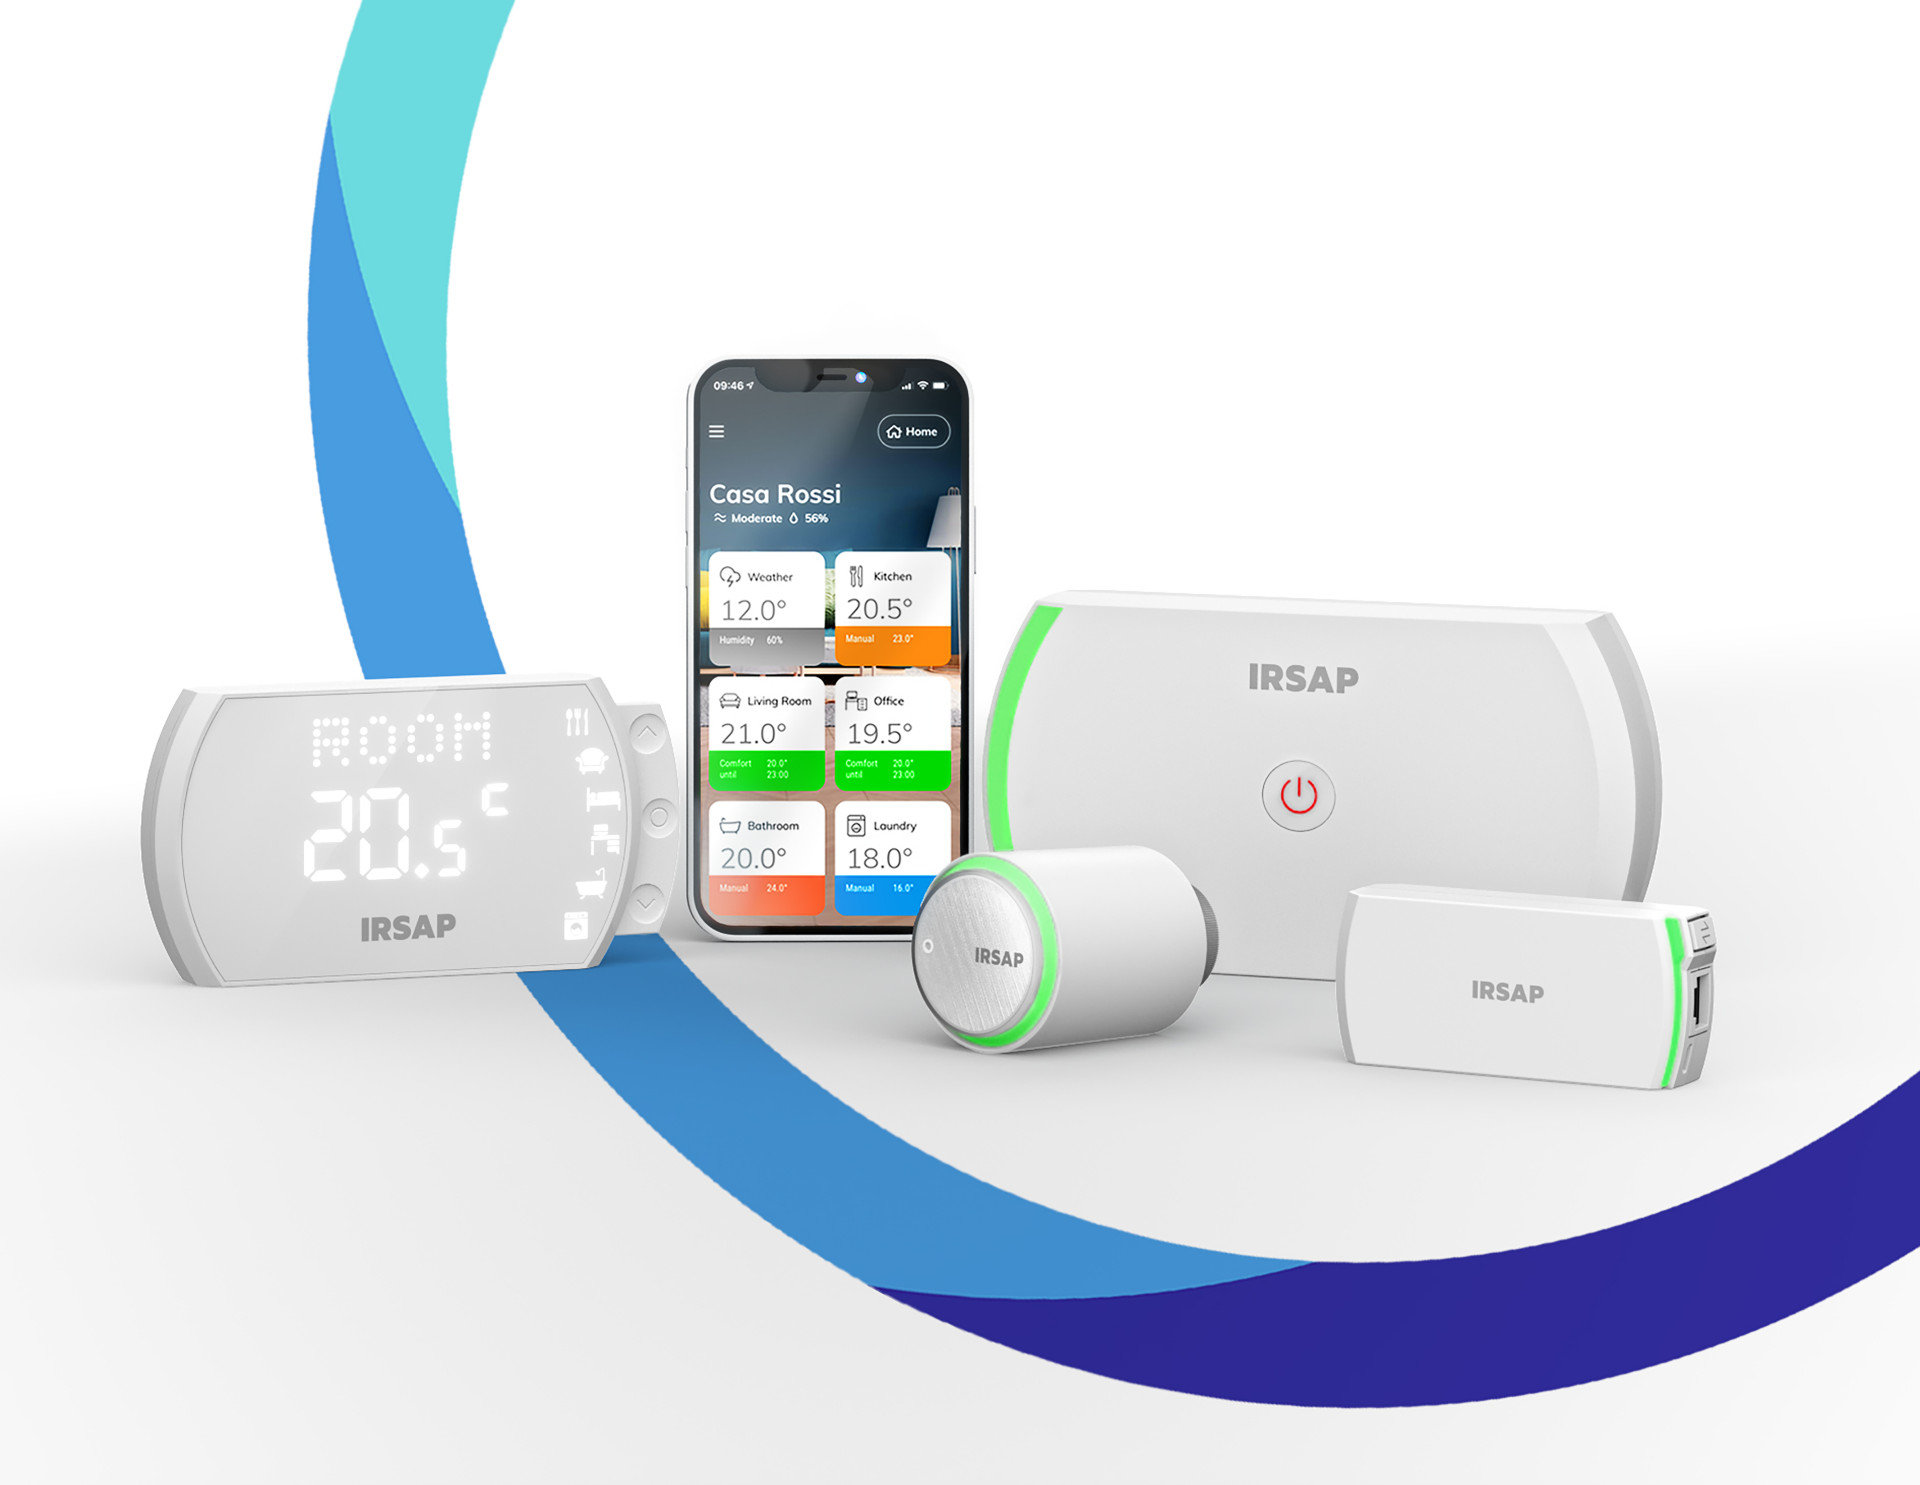
\includegraphics[width=11cm]{img/now.jpeg}
    \caption{Sistema IRSAP NOW per impianti idraulici}
    \label{fig:dispositivi_now}
\end{figure}

Una delle difficoltà attuali è l'impossibilità di andare a testare in maniera isolata i
dispositivi di questo ecosistema e l'unità centrale.

Ad esempio per validare una nuova versoine firmware della CU è necessario avere a disposizione tanti dispositivi quanti
ne supporta al massimo il sistema, ovvero 48, un numero che rende molto complessa anche a
livello logistico l'operazione (si pensi ad es. solo al fatto che questi dispositivi funzoinano a
batterie che dovrebbero essere continuamente mantenute cariche).

Si potrebbe quindi, mediante un'interfaccia radio opportunamente tarata sulle frequenze usate
dal sistema, andare a simulare i dispositivi lato software, consentendo con un'unica interfaccia
radio di simulare tutti i 48 dispositivi senza fisicamente averli in ufficio.

Oltre a ciò in questo progetto si può porsi anche ad un livello più basso: l'unità
centrale contiene due microcontrollori (e di conseguenza due firmware) che comunicano fra di
loro mediante un protocollo seriale (su interfaccia UART). Uno integra il ricetrasmettitore
a radiofrequenza ed è deputato a gestire la comunicazione con i dispositivi
finali, l'altro invece implementa tutte le logiche di funzionamento incluso l'interfacciamento
con il cloud, che avviene tramite porta ethernet.

Si potrebbe quindi andare a testare i due firmware in maniera isolata l'uno dall'altro,
andando a simulare sempre tramite software la controparte mancante. Questo evita di dover
testare tutto i sistema, in particolare la parte RF, quando uno solo dei due software viene
aggiornato. Infatti la parte radio viene aggiornata decisamente più di rado rispetto alla
gestione delle logiche di funzionamento, ma è la più dispendiosa in termini di tempo da testare
(anche perché gestendo a livello fisico la comunicazione RF, in linea teorica, ogni volta andrebbero
rieseguiti i test di laboratorio per assicurarsi che i parametri radio restino nei limiti
imposti dalla normativa vigente).

\subsection{Test di un termostato OpenTherm}

In IOTINGA infine abbiamo altri progetti firmware più complessi su cui questa metodologia
di test potrebbe essere applicata. Uno su tutti il progetto YAT (Yet Another Thermostat),
un cronotermostato Wi-Fi in grado di comunicare con la caldaia su bus OpenTherm.

La peculiarità di questo progetto è il fatto che è prevista l'interazione fra più
termostati mediante Bluetooth Low Energy (BLE). Quindi si potrebbe andare a validare
il funzionamento di un singolo esemplare andando a simulare gli altri dispositivi
che compongono la rete, oltre che simulare l'interazione con la caldaia OpenTherm
(esiste già uno strumento di test ufficiale prodotto dal consorzio che si potrebbe
integrare).

\end{document}
